 \section{Probabilidad condicional}

\begin{figure}[b]
	\centering
	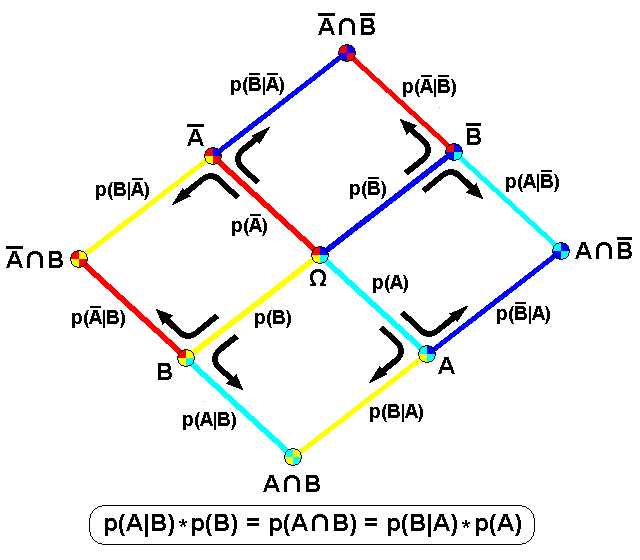
\includegraphics[width=0.7\linewidth]{images/Bayes_Theorem_2D}
	\caption{Diagrama para el teorema de Bayes.}
	\label{fig:bayestheorem2d}
\end{figure}


En esta sección, revisaremos el teorema de Bayes, el cuál describe un evento, basado en el conocimiento previo de las condiciones a las que está sujeto el problema. 

Para entender este teorema, necesitamos definir la probabilidad condicional, y como es que podemos usar los elementos de una partición para calcular la probabilidad de un evento.

Sean $A,B$ dos eventos tales que $P(A)>0.$
\begin{figure}
	\centering
	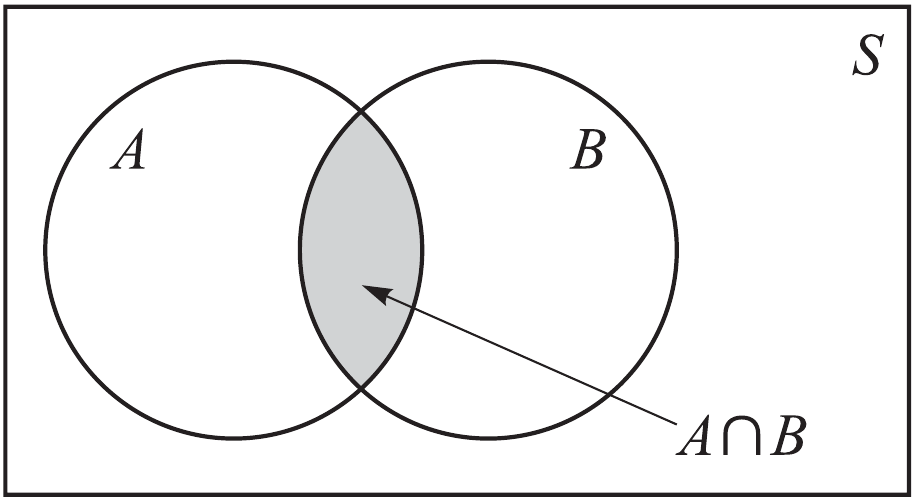
\includegraphics[width=5cm,keepaspectratio=true]{./pe/pands0103.png}
	% pands0103.png: 0x0 pixel, 300dpi, 0.00x0.00 cm, bb=
	\label{pands0103}
	\caption{Unión de dos conjuntos}
\end{figure}

Denotaremos por $P(B|A)$
la probabilidad de $B$ dado que $A$ haya ocurrido y diremos que es la \emph{probabilidad condicional} de $B$ dado $A.$


\begin{definicion}[Probabilidad condicional]
	\begin{align}
		P(B|A)&=\dfrac{P(A\cap B)}{P(A)} \\
		P(A\cap B) &= P(A)P(B|A)
	\end{align}
\end{definicion}


{}
\begin{observacion}
	La probabilidad condicional satisface todos los axiomas de una función de probabilidad.  Podemos pensar $P(\cdot|A)$ como la función de probabilidad que se obtiene al reemplazar el espacio muestral $S$ por $A.$
\end{observacion}

\begin{ejemplo}
	En un bote se colocan cinco canicas: tres blancas y dos negras. Inmediatamente después se agita el bote, con el fin de sortear su contenido.
	
	Determina la probabilidad de que en el segundo turno extraigamos una canica negra, dado que en el primero obtuvimos una blanca.  
\end{ejemplo}

\begin{solucion}
	Digamos que el evento $ E_i $ consiste en obtener una canica blanca en el í-esimo intento, de manera que $ E_i' $ es obtener una canica negra. 
	
	Entonces, la probabilidad de sacar primero una canica blanca y después una canica negra es 
	\begin{align}
		P(E_1\cap E_2') = \dfrac{3}{5}\times \dfrac{2}{4}=\dfrac{6}{20}.
	\end{align}
	Esto porque en el primer turno hay tres canicas blancas de cinco, pero si sacamos en una canica blanca (sin reemplazarla), entonces quedaran cuatro canicas, de las cuales dos serán blancas. 
	
	Ahora bien, la probabilidad $ P(E_1) $ de sacar una canica blanca al primer intento es $ \dfrac{3}{5} $, de manera que 
	\begin{align}
		P(E_2'|E_1) = \dfrac{1}{2}.
	\end{align}
\end{solucion}





{}
\begin{teorema}
	\label{thm:1.9}
	Para cualesquiera tres eventos $A_{1},A_{2},A_{3},$ tenemos que
	\begin{align}
		\label{1.19}
		P(A_{1} \cap A_{2} \cap A_{3})=P(A_{1})P(A_{2}|A_{1})P(A_{3}|A_{1} \cap A_{2})
	\end{align}
\end{teorema}


{}
\begin{teorema}
	\label{thm:1.10} Si $S=A_{1}\sqcup ... \sqcup A_{N},$  entonces
	\begin{align}
		\label{1.20}
		P(A)=P(A_{1})P(A|A_{1})+...+P(A_{N})P(A|A_{N})
	\end{align}
\end{teorema}


{}
Si $P(B|A)=P(B),$ i.e., la probabilidad de que $B$ ocurra no está afectada por la ocurrencia de $A,$ entonces diremos que $A$ y $B$ son independientes.


\begin{definicion}
	$A$ y $B$ son eventos independientes si y solo si
	\begin{align}
		\label{1.21}
		P(A \cap B) = P(A)P(B).
	\end{align}
\end{definicion}


{}
La definición se puede generalizar a más de dos eventos.  Por ejemplo, diremos que $A_{1},A_{2},A_{3}$ son eventos independientes si
\begin{align}
	k\neq j \rightarrow P(A_{j} \cap A_{k})=P(A_{j})P(A_{k}), \; j,k=1,2,3 
	\\ P(A_{1}\cap A_{2} \cap A_{3})=P(A_{1})P(A_{2})P(A_{3}).
\end{align}


%\begin{teorema}[Teorema de Bayes]
%	Si $S=A_{1}\sqcup A_{2} \sqcup...\sqcup A_{N},$ entonces
%	\begin{align}
%		\label{1.24}
%		P(A_{k}|A) = \dfrac{P(A_{k})P(A|A_{k})}{\sum_{j} P(A_{j})P(A|A_{j})}
%	\end{align}
%	
%\end{teorema}




